\chapter{RF Link}
The Link devices are communicating between each other through RF and this communication is maintained through what we call “RF Link” devices.  For this purpose, we have used the “CC1312R LaunchPad development kit” with CC1312R SimpleLink Sub-1 GHz wireless microcontroller unit. 

\begin{figure}[H]
\begin{center}
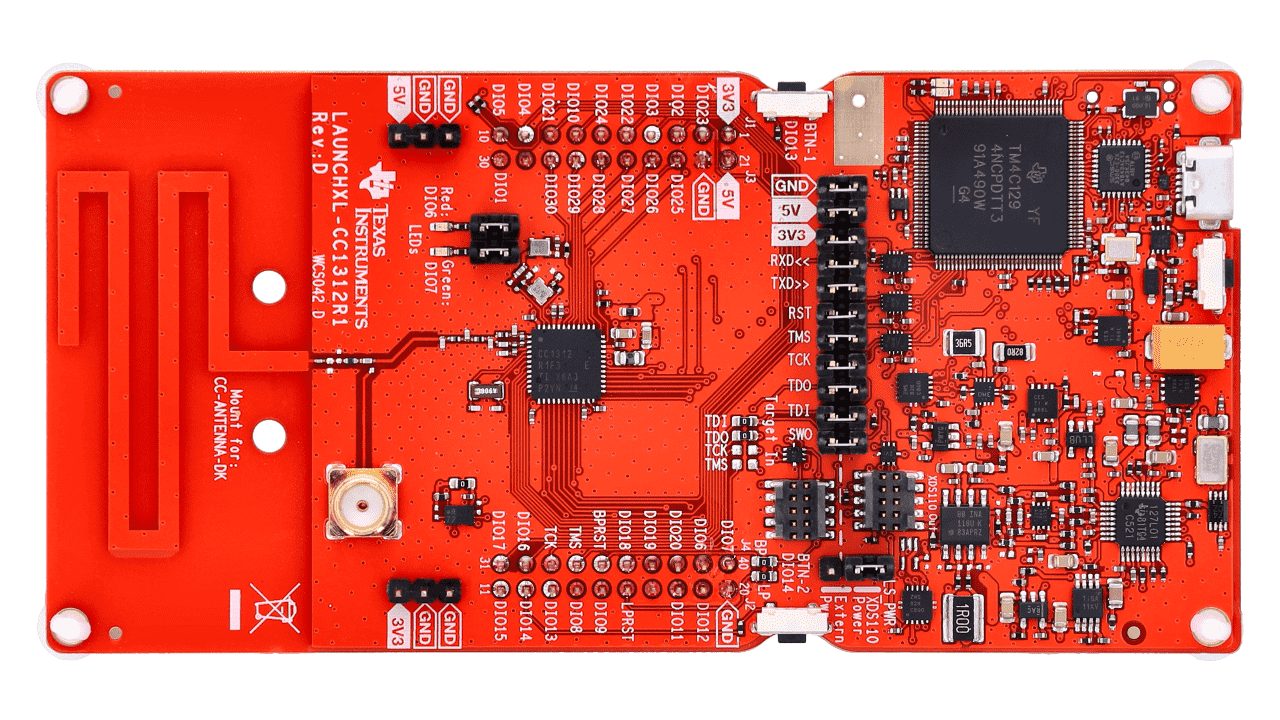
\includegraphics[width=0.90\textwidth]{cc1312r1-top}
\end{center}
\caption{Top view of CC1312R1}
\label{fig-pin}
\end{figure}

\begin{table}
\centering
\caption{Technical specifications of CC1312R1 MCU \cite{cc1312}}
\label{table1}
\begin{tabular}{|l|p{1cm}p{1cm}p{1cm}|}
\hline 
% \textbf{Name} & \textbf{Function} \tabularnewline
% \hline 
Main Processor & \multicolumn{2}{|c|}{48-MHz Arm Cortex-M4F} \tabularnewline \hline 
Programmable Flash & \multicolumn{2}{|c|}{352KB} \tabularnewline \hline 
ROM for protocols and library functions & \multicolumn{2}{|c|}{256KB} \tabularnewline \hline 
SRAM cache & \multicolumn{2}{|c|}{8KB} \tabularnewline \hline 
Ultra-low leakage SRAM & \multicolumn{2}{|c|}{80KB} \tabularnewline \hline 
\multicolumn{3}{|c|}{ Flexible high-performance sub-1 GHz RF transceiver } \tabularnewline \hline 
RF coprocessor & \multicolumn{2}{|c|}{Arm Cortex-M0} \tabularnewline \hline 
Separate SRAM & \multicolumn{2}{|c|}{16KB} \tabularnewline \hline
\multirow{3}{*}{Frequency Bands} & \multicolumn{2}{|c|}{143 MHz to 176 MHz}  \tabularnewline
{} &  \multicolumn{2}{|c|}{359 MHz to 527 MHz} \tabularnewline 
{} &  \multicolumn{2}{|c|}{861 MHz to 1054 MHz} \tabularnewline \hline
Sampling Rates & \multicolumn{2}{|c|}{2.5 kbps to 1000 kbps} \tabularnewline \hline 
Modulation Type & \multicolumn{2}{|c|}{2-FSK, 2-GFSK} \tabularnewline \hline 
\multirow{3}{*}{Receiver sensitivity} & \multicolumn{1}{|c|}{2.5 kbps (Long Range Mode)} &  \multicolumn{1}{|c|}{-121 dBm} \tabularnewline 
{} & \multicolumn{1}{|c|}{50 kbps} & \multicolumn{1}{|c|}{-110 dBm} \tabularnewline
{} & \multicolumn{1}{|c|}{1000 kbps} & \multicolumn{1}{|c|}{-97 dBm} \tabularnewline \hline 
Maximum Output power & \multicolumn{2}{|c|}{+14 dBm \newline (with temperature compensation)} \tabularnewline \hline  
\end{tabular}
\end{table}

\newpage

\section{Brief Description of RF Link's Radio Configuration}

First of all, if we want to transmit data over radio, we must choose a certain modulation scheme. The best option, for the ranges we intend to support, that CC1312R supports is 2-GFSK. All the work related to the modulation is handled by the MCU’s RF Core.
Taking this into consideration, we would not go deep into its inner workings, but very briefly: Frequency-Shift Keying (FSK) is a frequency modulation scheme in which digital information is encoded on a carrier signal by periodically shifting the frequency of the carrier between several discrete frequencies. GFKS is an extension of FSK where Gaussian filter is used to reduce the abrupt changes in frequency, resulting in a continuous phase and a bandwidth-efficient signal. 2 in 2-GFSK refers to the number of tones (frequencies with certain deviation from our carrier frequency) used to encode the signal. Table \ref{rf-link-config} presents the RF characteristics selected for our application. 

\newpage

\begin{table}
\centering
\caption{RF Link Radio Configuration}
\label{rf-link-config}
\begin{tabular}{|l|l|}
\hline 
Carrier Frequency & 868 MHz \tabularnewline \hline 
Symbol Rate & 1000 kBaud \tabularnewline \hline
Modulation Format & 2-GFSK \tabularnewline \hline
Frequency Deviation & 350 kHz \tabularnewline \hline
RX Filter Bandwidth & 2185.1 \tabularnewline \hline
\end{tabular}
\end{table}

\begin{table}
\centering
\caption{RF Packet Structure}
\label{rf-pkt-struct}
\begin{tabular}{|l|l|l|l|l|}
\hline 
Preamble & Sync Word & Length Byte & Payload & CRC \tabularnewline \hline
4 bytes & 4 bytes & 1 byte & 1 - 255 bytes & 2 bytes \tabularnewline \hline
\end{tabular}
\end{table}

The preamble in the proprietary PHY consists of an alternating bit pattern 0101... and is used to determine the amplifier gain. Unlike in older TI devices, it is not needed for the bit synchronization (Cite Packet Format Documentation). 
The sync word is used by the packet engine to detect the packet start, meaning it has a similar purpose to the start delimiter in Interlink packets. The value for the sync word is selected such that it has high self-correlation. We are using the default sync word for CC1312R: 0x930B51DE.
As we are using variable length packets, the length byte is automatically added by the transmitter, so that receiver will know the number of bytes expected in the payload.
At the end of the packet CRC is added, which is used to detect when a packet is received with errors.

\section{Interaction with RF Core Coprocessor}

As it has already been mentioned the inner workings of RF Core of CC1312R MCU are abstracted away and we are interacting with it through TI’s drivers. There are 3 commands we have used:
\begin{enumerate}[nolistsep]
\item CMD\_FS - Sets frequency and start the synthesizer 
\item CMD\_PROP\_TX - Used to pass transmission related commands to the RF core 
\item CMD\_PROP\_RX - Used to pass reception related commands to the RX core 
\end{enumerate}

One important remark is that RF Core’s controller has a separate built-in RAT (Radio Timer), which is used for the accurate timing of the command execution. This timer would not be affected by the execution of our main program, which is crucial for maintaining correct timings as it will become apparent later.

The commands can be given to the RF core in various ways - the 3 most important ones being:

\begin{enumerate}[nolistsep]
\item Abort all current operations and immediately proceed to the execution of the given command,
\item Append the given command to the current execution chain to be executed after all the currently queued radio operations are finished,
\item Schedule a command to be executed with precise timing, which is given in RAT timer ticks. This one is especially important, because things like transmission operation need a “warm-up” time to reach the state when the transmission can begin. This is crucial as by scheduling a command at a precise time, the RF core processor would perform the “warm-up” beforehand to start the transmission precisely at the specified time.
\end{enumerate}

\section{Time-Division Multiple Access Configuration}

As our RF link agents have to share a communication medium (i.e., air, as we are using RF), we must employ some sort of channel access method. The method we have chosen is Time-Division Multiple Access (TDMA), where agents have dedicated time slots for transmission. In our case, we have settled on building a half-duplex communication system, where the parties can communicate bidirectionally, but not simultaneously. As currently we only have enough hardware on hand for two RF devices, we decided to organize time division in the following manner: one of the RF devices will take the role of the “master" and the other will be assigned the role of the "slave." 
The roles are assigned based on the state of the GPIO pin DIO25. This pin is operating in pull up mode, so if we connect it to ground with a jumper, the value of the pin will become 0, meaning it will be the \emph{slave}.
Based on the initialized roles, both of the agents know their designated time slots, assuming they have synchronized clocks. Moreover, we are using roles in the process of the clock synchronization as the \emph{slave} adjusts its clock based on the \emph{master’s} clock (this process will be examined in more detail later). Each time slots has a duration of 2500 microseconds, during which one of the parties will transmit and the other will receive. The time slots are virtually divided into odd and even numbers, the \emph{master} device will transmit data (if data is available) in even time slots and \emph{slave} device will transmit data in odd timeslots. As long as both devices have synchronized time slot timer (system clock), they should not transmit data at the same time (so that transmitter collision will be avoided).
\begin{figure}[H]
\begin{center}
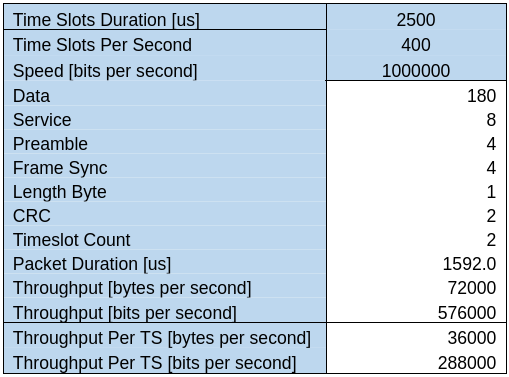
\includegraphics[width=0.60\textwidth]{TDMA}
\end{center}
\caption{TDMA Characteristics}
\label{tdma-chrac}
\end{figure}

The throughput of each timeslot is 36000 bytes per second, the UART speed (described in the section below) is 230400 bauds, which corresponds to 23040 bytes per second. As a result, the bottleneck of the system is not in the RF communication, but rather the UART link. 

\section{RF Link's Connection to Link Device}

We will communicate with the “Link device” through UART. We encountered an issue with our MCU’s UART not working properly with non-standard baud rates. The baud rate of the UART is set to 230400 bauds per second as the processing power of our chip was not sufficient to handle processing data if we increased the baud rate to the next standard value of 460800. This is unfortunate, as the throughput of our RF should have been sufficient for higher data rates, but our chip was unable to handle the processing of so much data. As in the case of the “Link device’s” UART connection, we are using DMA to offload some work from our processor. Fortunately, TI’s drivers simplify the process a lot, and the only thing left for us to do is to oscillate between the two buffers of the maximum RF packet payload size (180 bytes) on reception callback. 

\section{RF Link Timer}

At the initial boot-up of the RF link module, we start a 16 bit timer with a period of 10 microseconds. We set its interruption priority to 1 (highest possible), so we can use this as a main system clock. 
We maintain 2 tick counters (“system time tick” and “self time tick”). In the case of the \emph{master}, these 2 tick counters are equivalent, but for the \emph{slave}, “self time tick” counter is used to keep its own time, while the “system time tick” is going to be synchronized with the \emph{master’s} time to ensure that the time slot rotations are simultaneous for all parties. Moreover, during every timer interrupt callback, we check if we have reached the current device’s transmission time slot. If so, in a case of having data to be transmitted, we perform the following 3 operations:
\begin{enumerate}[nolistsep]
    \item Set a flag that indicates the need for processing an upcoming TX packet. We do not perform the processing of the upcoming TX packet at the interrupt itself, as we do not want to block the program execution flow in the interrupt,
    \item Fix the current system tick counter in the variable "txSyncTick". This is only being used in the case of the \emph{master} as it must share its time for the other parties in the network to adjust their system times according to it,
    \item Calculate the transmission start time. It is calculated as: \[ \text{Current\ RAT\ Time + TX\_CMD\_TO\_START,} \] where “TX\_CMD\_TO\_START” is the time that would be sufficient for the RF core to reach the state of readiness for transmission. Also, having a margin before the start of the packet transmission allows us to have lower time synchronization accuracy.
\end{enumerate}

\section{RF Link Packet Structure}


\begin{table}
\centering
\caption{RF Link Packet Structure}
\label{rf-link-pkt-struct}
\begin{tabular}{|p{1in}|p{1.5in}|p{2in}|} \hline 
\multirow{4}{*}{Header} & Packet type & {1 byte unsigned integer} \\ \cline{2-3}
 & Packet ID & 1 byte unsigned integer \\ \cline{2-3}
 & Payload length & 2 byte unsigned integer \\ \cline{2-3}
 & System tick value & 4 byte unsigned integer \\ \cline{2-3} \hline
 \multicolumn{2}{|c|}{Payload} & Max 180 bytes \\ \hline
\end{tabular}
\end{table}

When designing the initial structure, we have devised 2 packet types (service and data), but currently we have no use for the service packets. The same situation occurs with IDs as we do not use them either, but the IDS are intended to later be used to facilitate the ability to request the repetition of corrupted or missed packets.

\section{RF Transmission Procedure}

On every cycle of the program's execution loop, we check if any data has been received via UART and if so, we prepare a radio packet to be transmitted when the current party's transmission time slot begins. The packet is enqueued to the transmission queue, and we have its maximum length set at 10. As the speed on RF communication is higher then the speed of UART communication, this queue should never reach its maximum length. 
If during the execution loop our program encounters the flag that indicates the need for processing an upcoming TX packet being set, it performs a procedure represented by the following pseudo code:

\lstset{language=c, showstringspaces=false, tabsize=1, breaklines=true, breakatwhitespace=false, framexleftmargin=20pt,numbers=left, 
numberstyle=\small,numbersep=10pt,frame=single,captionpos=t,xleftmargin=.061\textwidth}
\begin{center}
\begin{lstlisting}[caption=RF Transmission Preperation Procedure, label=nodemcuconfig]
start_time <- RF_getCurrentTime()
fixTickCounter()
RF_cancelOngoingCommand()
txPacket <- getCurrentTXPacket()
txPacket.header.tick <- txSyncTick
RF_sendPacket(txPacket)
RF_startReception()
resumeTickCounters(RAT_TO_SYSTICK(RF_getCurrentTime() - start_time))
processTxPacketFlag <- false
\end{lstlisting}
\end{center}

The drivers that TI provides are written in such way that all interrupts are disabled during the process of passing the command to RF core. As this would mess up our tick counter, we had to come up with a workaround. The workaround consists of stopping the timer at the beginning of the procedure and at the end of the procedure resuming it after fixing the tick values using the time difference measured using the RAT, which is unaffected by disablement of interrupts as it runs on the RF core. It is carried out in the lines 1, 2, and 8. It is important to note that in the "RF\_sendPacket" sub procedure we send the transmission command to the RF core with the scheduled time calculated when \emph{processTxPacketFlag} was set. At the end, we send a new command to RF core to start reception, which would queue in the command chain, as there is no reason to stay in transmission mode after the data has been sent, i.e., the previous command for transmission had been finished executing. 

\section{RF Reception Procedure}

The TI driver for RF core provides the ability to register a callback on the data reception. We are interested in two events:
\begin{enumerate}[nolistsep]
    \item \emph{RF\_EventRxOk}: occurs when a packet reception has finished,
    \item \emph{RF\_EventRxEntryDone}: occurs when the last packet that was received is available to be read.
\end{enumerate}

In the case of the first event occurring we just fix the tick value in the “rxRdyTick” variable. In case of the second event, we read the packet from the RFQueue (provided in the TI drivers) and enqueue it in our internal rx packet queue with its “rxRdyTick”. On the next iteration of the program’s loop we send the packet’s payload to the Link device through UART. If the receiving device has the role of the \emph{slave}, it proceeds to system tick adjustment procedure.

\section{RF Synchronization Procedure}

First, we must calculate the time in ticks that has passed since we have received the packet. We do so by subtracting the “rxRdyTick” from the current value of the tick counter and store it in “rxTickPassed”. Then we calculate the packet transmission duration. Below is the formula for its calculation:

\begin{equation}
t_{packet} = \frac{(N_{preamble} + N_{syncword} + N_{length} + N_{CRC} + N_{header} + N_{payloadLength}) \times 8}{\text{Data Speed}} \times 1000000
\end{equation}

Where:
\begin{enumerate}[nolistsep]
    \item \(N_{preamble}\): number of bytes in the preamble (4 in our case),
    \item \(N_{syncword}\): number of bytes in the sync word (4 in our case),
    \item \(N_{length}\): number of bytes of the packet length field (this is automatically calculated and added by RF core) (1 in our case),
    \item \(N_{CRC}\): length of CRC in bytes  (2 in our case),
    \item \(N_{header}\): length of our packets header in bytes (8 in our case),
    \item \(N_{payloadLength}\): length of our payload in bytes (0-180 in our case),
    \item \(N_{preamble}\): number of bytes in the preamble (4 in our case),
    \item Data Speed: Symbol Rate, meaning number of symbols (in case of 2-GFSK, bits) per second (1,000,000 in our case),
\end{enumerate}

The part of the equation in the bracket is the length of the whole RF packet in bytes. We multiply it by 8 to get the number of symbols (bits). Then we divide it by "Data Speed" to get the duration of the packet in seconds and then multiply it by 1,000,000 to convert it to microseconds. After we have obtained the packet duration, we can calculate the new adjusted system tick.

\begin{multline}
\text{system tick = } tick_{rxHeader} + \frac{\operatorname{RatTicksToUs} (tick_{cmdToStart} + tick_{startToPreamble})}{N_{usInTick}} \\  + \frac{t_{packet}}{N_{usInTick}} + rxTickPassed + \frac{100}{N_{usInTick}}
\end{multline}

Where:
\begin{enumerate}[nolistsep]
    \item \(tick_{rxHeader}\): the tick value of master's system tick on its transmission slots beginning,
    \item \(tick_{cmdToStart}\): the time between the beginning of the time slot and the start of transmission in RAT ticks,
    \item \(tick_{startToPreamble}\): the time between the start of transmission process and the start of preamble being sent (the time when data physically starts to transmit),
    \item \(RatTicksToUs\): RAT ticks to microseconds conversion operation,
    \item \(N_{usInTick}\): number of microseconds in one tick. We divide by it the microseconds values to get the value in ticks.
\end{enumerate}

The last part of the equation may seem bizarre. We have found it experimentally, by looking at the difference between the clocks of \emph{master} and \emph{slave} with an oscilloscope even after adjustment. The reason for the constant error is possibly the RF signal demodulation process. This includes data demodulation, CRC calculation and copying of the data from internal buffers to the reception queue for outputting data from RF core.
It may seem unnecessary to adjust the clock on the \emph{slave} on every received packet, but it is very important because every crystal oscillator (which is used to generate the operational clock of the microcontroller, and as a result the system timer) has some inaccuracy and the inaccuracy can differ from one crystal oscillator to another and even though the inaccuracy may seem insignificant, it can add up over time causing drift between the agents' clocks if we just adjust them once.

\begin{figure}[H]
\begin{center}
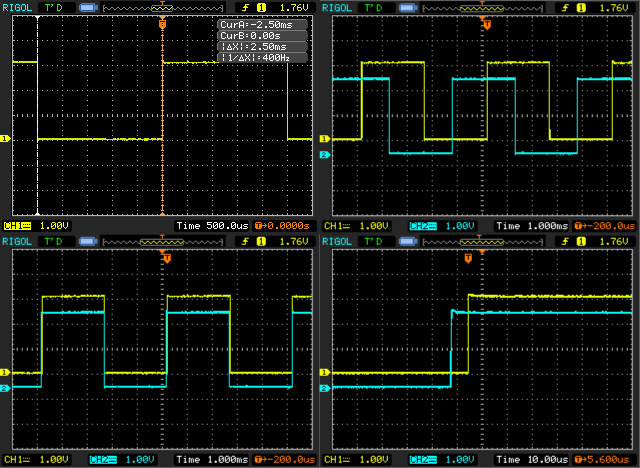
\includegraphics[width=0.90\textwidth]{time-slots.png}
\end{center}
\caption{Screenshots of oscilloscope showing the time slots, where lows are the odd time slots, and the highs are the even time slots. (top left) Measurement of the duration of single time slot. (top right) Signals from \emph{master} and \emph{slave} device before synchronisation. (bottom left) Signals from \emph{master} and \emph{slave} device after synchronisation. (bottom right) Close-up of the signals from \emph{master} and \emph{slave} device after synchronisation. }
\label{fig-oscilloscope}
\end{figure}

As it can be seen in the right bottom section of \ref{fig-oscilloscope}, even after the synchronisation, we have approximately 7 microseconds of discrepancy between clocks. This is expected as timers on RF Links run with 10 microseconds period, so our error theoretically can't be lower then that. However, even with this 10 microseconds of error, our synchronisation procedure yields results that are more than sufficient to maintain a reliable operation of our system.  


% The NodeMCU parameters are listed in Table \ref{table2}.

% \begin{table}
% \caption{Parameters of NodeMCU}
% \label{table2}
% \centering
% \begin{tabular}{|l|p{3.7cm}|p{4.8cm}|}
% \hline 
% \textbf{Categories} & \textbf{Items} & \textbf{Values} \tabularnewline
% \hline 
% \multirow{1}{*}{Wi-Fi Parameters} & certificates & FCC/CE/TELEC/SRRC \\\cline{2-3}
%                  & WiFi Protocols & 802.11 b/g/n \\\cline{2-3}
%                  & Frequency Range	 & 2.4G-2.5G (2400M-2483.5M) \\\cline{2-3}
%                  & \multirow{2}{*}{TX Power} & 802.11 b: +20 dBm \\\cline{3-3}
%                  & & 802.11 g: +17 dBm \\ \cline{3-3}
%                  & & 802.11 n: +14 dBm \\ \cline{2-3}
%                  & \multirow{2}{*}{RX Sensitivity} & 802.11 b: -91 dbm (11 Mbps)   \\\cline{3-3}
%                  & & 802.11 g: -75 dbm (54 Mbps)  \\ \cline{3-3}
%                  & & 802.11 n: -72 dbm (MCS7) \\ \cline{2-3}
%                    & Types of Antenna & PCB Trace, External, IPEX Connector, Ceramic Chip    \\ \cline{1-3}
                 
% \multirow{1}{*}{Hardware Parameters} & \multirow{2}{*}{TX Power} & UART/SDIO/SPI/I2C/ \newline I2S/IR Remote Control \\\cline{3-3}
%                  &  & GPIO/PWM\\\cline{2-3}                
%                  & Operating Voltage & 3.0~3.6V \\ \cline{2-3}
%                  & Operating Current & Average value: 80mA \\ \cline{2-3}
%                  & Operating Temperature Range& -40°~125° \\ \cline{2-3}
%                  & Ambient Temperature Range & Normal temperature  \\\cline{2-3}
%                  & Package Size & 5x5mm  \\ \cline{2-3}
%                  & External Interface & N/A \\ \cline{1-3} \hline 
% \end{tabular}
% \end{table}
